\documentclass{report}
\usepackage[utf8]{inputenc}
\usepackage[top=2.5cm, left=2.3cm, right=2.7cm, bottom=3.0cm]{geometry}
\usepackage{accents}
%\usepackage{amsmath}
\usepackage{float}
\usepackage{hyperref}
\usepackage{pdfpages}
\usepackage{sectsty}
\usepackage{titlesec}
\usepackage{listings}

\titleformat{\chapter}{\normalfont\huge}{\thechapter.}{20pt}{\huge}
\newcommand{\ubar}[1]{\underaccent{\bar}{#1}}
\newcommand{\e}[1]{\cdot10^{#1}}


\title{Main Coursework \\ Computational Intelligence \\ COMP-575}
\author{Tudor Jianu [201532511]}
\date{07-05-2021}
\usepackage{graphicx}
\begin{document}

\maketitle

\chapter{Perceptron}
The Perceptron is a simple error correction algorithm that aims at fitting a line called decision boundary that separates the given classes. The Perceptron is able to learn by correcting its output through the adjustment of weights such that the output equals the target. 
Generally, the weights of the Perceptron are initialised to zero although in this implementation made use of the NumPy random library and generated a set of weights in the $(0,1]$ interval while the learning rate $\eta$ has been made available to the user to select it. The activation function implemented has been a simple sign function that maps the values of $z=W(t)^{T} x(t)$ based on the sign as:

 




\begin{figure}[htp]
\centering
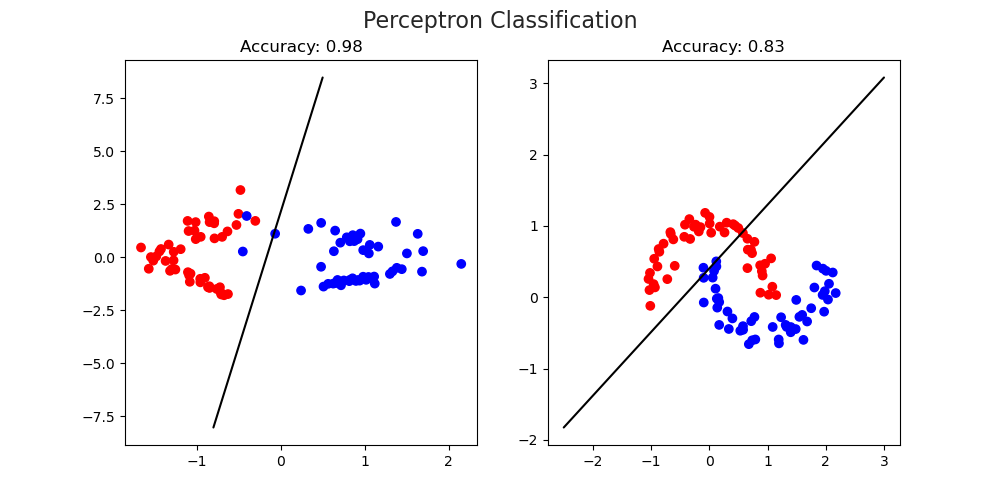
\includegraphics[scale=0.70]{Perceptron/Perceptron.png}
\caption{Perceptron}
\label{Perceptron}
\end{figure}




\chapter{Multi-Layer Perceptron}

\subsection{}

\chapter{Evolutionary Optimisation}
\section{Genetic Algorithms}

\subsection{Simple-GA}

\begin{figure}[htp]
\centering
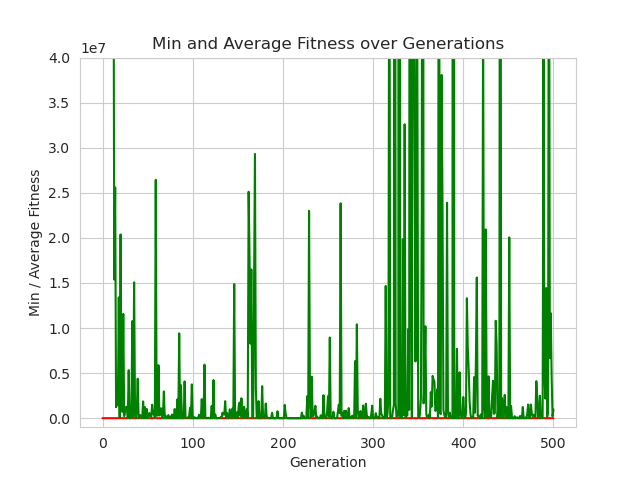
\includegraphics[scale=0.80]{Genetic/Simple.png}
\caption{GA}
\label{GA}
\end{figure}

\subsection{Elitism}
\begin{figure}[htp]
\centering
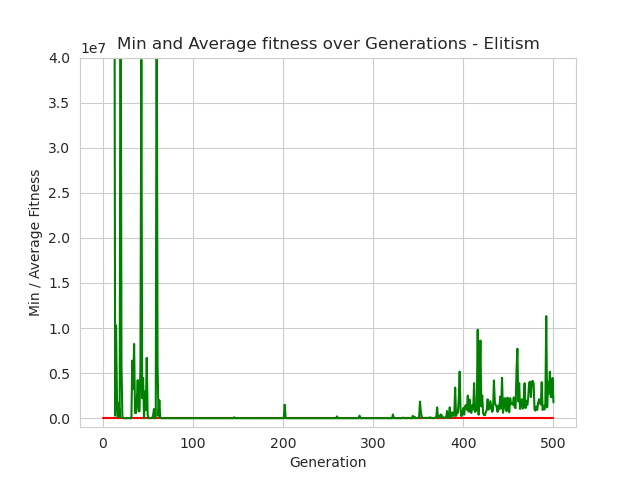
\includegraphics[scale=0.80]{Genetic/Elitism.png}
\caption{GA-Elitism}
\label{GA-Elitism}
\end{figure}

\section{Particle Swarm Optimisation(PSO)}



\include{1}
%\include{code}
%\bibliographystyle{abbrv}
\bibliography{references}

\end{document}